\section{Facility}
\label{sec:facility}
%Because of these reasons this experimental facility will be created. \\
Existing flumetank is used \\
ALL INFO ABOUT EXISTING FLUMETANK \\
A schematic of the tank is shown in HIER EEN FIGUUR VAN DE BESTAANDE FLUMETANK MET AFMETINGEN. 


\subsection{Wavemaker}
\label{sec:wavemaker}
Wavemaker: some design conditions \\
1: has to operate in flow (no obstruction but still good waves) \\
2: has to operate within the dimensions of the tank \\
3: has to be able to make regular and irregular waves \\
Plunging wedge type wavemaker. based in theory developed over the years by \citet{Madsen1970,Wu1988,Lowell2020} \\
Designed for waves of a length between 0.05 meter and 3 meter with a maximum wave height over length of 1/25. These values are chosen because at maximum water depth the waves will be deep water to intermediate gravity waves in this range. \\
These design choices have led to the wavemaker shown in figure \ref{fig:exp_wavemaker}. The maximum amplitude of the stroke of the wavemaker is 0.12 m and the maximum velocity is 0.6 m/s. To move and control the wavemaker a servo motor (EMMT-AS-80-M-HS-RSB). servo motor controller (CMMT-AS-C3-11A-P3-EP-S1) and electric cylinder (ESBF-BS-50-300-10P-S1-R3)  are used. 

\begin{figure}
	\centering
	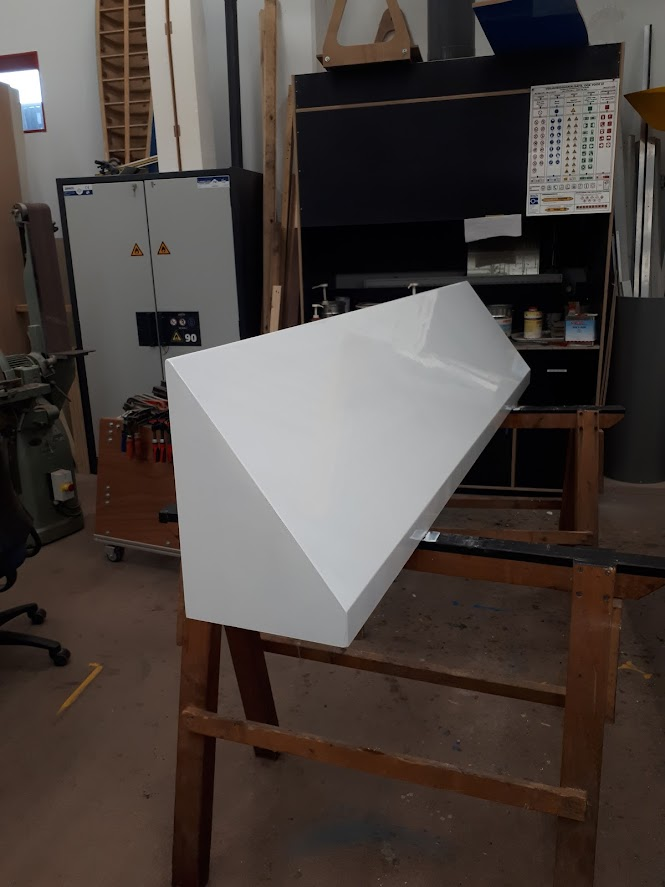
\includegraphics[width=0.8\linewidth]{figs/Wedge_wavemaker_painted.jpg}
	\caption{PLACEHOLDER The wavemaker, placed to generate waves}
	\label{fig:exp_wavemaker}
\end{figure}

\subsubsection{Waves wavemaker}
\label{sec:results_wavemaker}
To be able to generate the waves that we want to generate, we need to know how well the wavemaker works. This will be tested by systematically testing the wavemaker and measuring the results.
HIER OVERZICHT VAN GOLVEN DIE GEMETEN GAAN WORDEN (CONSTANT/SPREIDING. MAX. MIN. ONREGELMATIG)
%WAVESPECTRUM JONSWAP BUT CUTOFF FOR FREQUENTIES ABOVE 6Hz. THESE ARE CAPILLARY WAVES AND ALSO THE HIGH FREQUENCY TALE. LESS RELEVANT (this is the case for the P Wellens files)

\subsection{Beach}
\label{sec:beach}
To minimize reflections which will interfere with the created waves. the waves should be dissipated as much as possible once they have moved passed the model.
For this a dissipation device, also called a beach, is used. It is shown in figure \ref{fig:exp_beach} \\
\begin{figure}
	\centering
	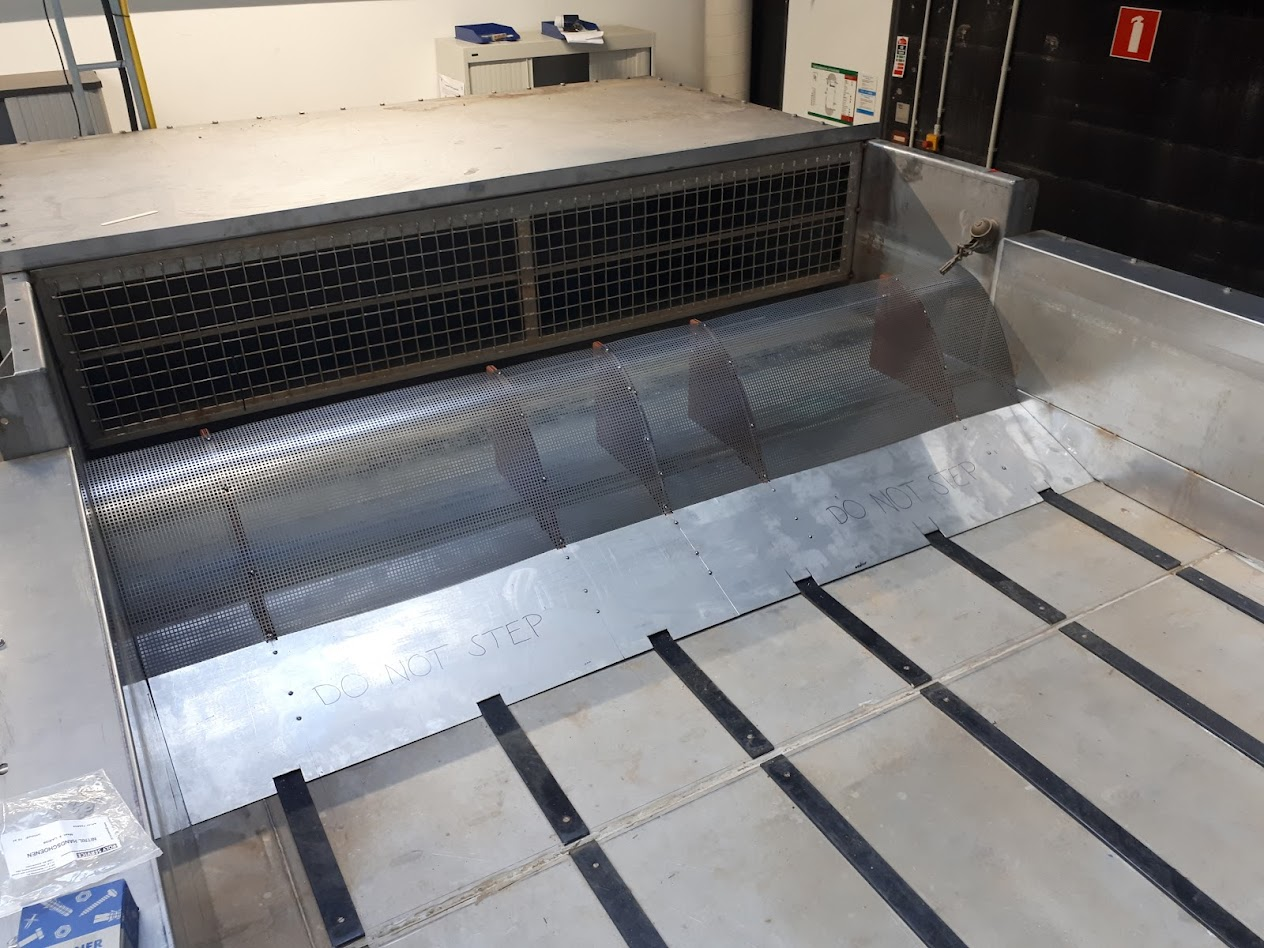
\includegraphics[width=0.8\linewidth]{figs/Picture_beach.jpg}
	\caption{PLACEHOLDER The beach, placed to dissipate wave energy}
	\label{fig:exp_beach}
\end{figure}


Instead of making this beach impermeable. it is more effective to introduce perforations help dissipate wave energy. The size of the perforations for the beach were based on the research by \citet{Chegini1994}. The beach is made of 1 mm thick stainless steel with 5 mm wide squares and a total perforation rate of 45\%.  \\
For the shape of the beach a parabola was chosen. From a survey conducted by \citet{Ouellet1986} the parabolic shape profile was recommended. Based on the results found in \citet{Hodaei2016} and scaling those to our experiments. a parabolic shape of $y = -3.32 \cdot x^2 + 0.04\cdot x$ was chosen. The beach is placed such that the highest point is at the waterline. The scaling and design of the beach is done with a focus on long waves. This because for the longest waves the largest reflection coefficients are found. as shown in \cite{Suh2003}. They also contain more energy compared to shorter waves of similar steepness. Also. they move faster thus could actually be able to move towards the model even if there is current. and they have the highest chance of influencing the results. Because of all these reasons the focus during the designing of the beach has been on damping these largest waves.

\subsubsection{Effectiveness beach}
\label{sec:results_beach}
To see how effective the beach is, thorough measurements will be conducted with various regular and irregular waves, and various current velocities. The reflection coefficients for different waves and wave spectra should be known as this will pollute the generated wave spectra during long running experiments.

\subsection{Validation facility}
\label{sec:validation_facility}
Tests are conducted in the towing tank in an irregular wave spectrum. These experiments will be repeated in the wave-current tank to validate the testing facility.

\subsection{Data handling}
\label{sec:data_handeling}
Goal of test facility is to create large amounts of data, but this data also needs to be saved, stored and processed. The data acquisition flow is visualized in figure \ref{fig:exp_data_flow}. 
Video footage is obtained and saved using the open source software Open Broadcaster Software (OBS). This, together with the acquired data can be viewed live during the experiments, allowing for active supervision.



\begin{figure}
	\centering
	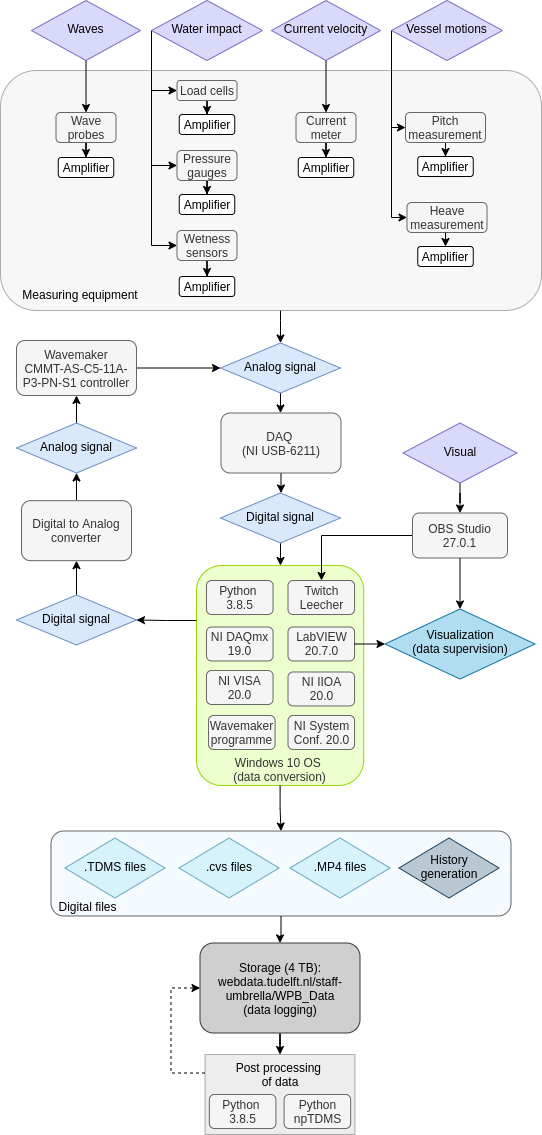
\includegraphics[width=0.8\linewidth]{figs/Data_acquisition_flow.drawio.png}
	\caption{Flow of the data during experiments, from acquisition to storage}
	\label{fig:exp_data_flow}
\end{figure}




\subsubsection{Data analysis}
\label{sec:analyzing_data}
To find the events the wetness sensors are used \\
EXPLAIN HOW I HANDLED ALL THE DATA


\section{Experiments}
\label{sec:exp}

\subsection{Chosen conditions}
\label{sec:exp_conditions}
The peak frequency and significant wave height are based on rough sea conditions or storm conditions found in sources \cite{Deelen2014, Mazaheri2019, Collins2018, Techet2005}. \\

At full scale the depth would be about ......... This might seem unrealistic as the average of the worlds oceans is 3729 m \cite{Zeecijfers}. The North Sea and Gulf of Thailand however. areas with a lot of ship traffic. have respectively and average depth of 95 m \cite{NorthSeaDepth} and 58 m \cite{Khongchai2003}. This shows that the wave conditions where bottom effects play some role are not unreasonable.

